%Even if historically customers still think they are connected to the Internet using a simple modem, the truth is that broadband connection is delivered by a full-fledged HG, integrating the functions of a modem, network address translation (NAT) router, Ethernet switch, WiFi access point, DHCP server, firewall, among others.
 
%No standard technical specification has been defined for HG. However a set of Functional Requirements is maintained by the Broadband Forum in TR-124 \cite{broadband_forum_functional_2014}.
The following section will present the most common architectures for HGs.
A special interest will be shown for execution environments, which are meant to achieve modularity through the Service Oriented Programming (SOP) paradigm \cite{bieber2001introduction}.


\subsection{Architecture and execution environment for the Home Gateways}

\subsubsection{Firmware based HG}
HG's firmware is a custom proprietary embedded system software deployed by vendors into their devices.
This solution is still widely used by vendors, but lacks the ability to act as a real execution environment.
Even if Service Providers or End-Users can alter its configuration, new services cannot easily be deployed on-the-fly.
A complete system update by the Service Providers is necessary to deploy new features.
   
\subsubsection{GNU/Linux HG}
   
GNU/Linux is also used as a platform of choice for Home Gateways \cite{royon_multiservice_2007}.
The solution is considered stable, tested and allows reusing well-known applications for networking, among others.
After Linksys (a router vendor who published its GNU/Linux based firmware designed for its WRT54G product line in 2003), a lot of efforts have been made to maintain and improve embedded GNU/Linux firmware distribution over a wide variety of platforms.
A notable example is the OpenWrt\footnote{https://openwrt.org/} project which has been partly sponsored among others by Comcast, through the Open Home Gateway Forum.
%It has helped researchers to add new features to commodity routers by replacing the firmware with a real GNU/Linux OS along with a file system and a package management tool.
%In addition of being able to deploy new packaged programs, developers can also use OpenWrt to write their own applications and deploy them in production.

Modularity can be achieved within the GNU/Linux platform.
The large application catalog available, usually benefits from low memory consumption and low IO footprint.
However, programs must be cross platform and Service Oriented Architecture is not natively supported.
Due to this, alternative execution environments such as OSGi are promoted.


   
\subsubsection{HG with OSGI execution environment}
   
OSGi is a specification that describes a modular system and a service platform for Java.
It was originally designed to enable the deployment of services over wide area networks to local networks and devices (\cite{marples_open_2001}).
The main advantages of OSGI are platform and application independency, multiple services support and collaboration by letting services discover each other and adapting their behavior accordingly.

The Home Gateway Initiative (HGI)\footnote{http://www.homegatewayinitiative.org} publishes Requirements  proposing an architecture for Modular HG \cite{_requirements_2011}, \cite{_hg_2014}.
It explicitly indicates OSGi as the solution of choice to deploy additional modules in their HGI Open Platform 2.0.
This deals with the modularity issues of the latter approaches.
For HGI, the goal for OSGi is to allow the installation, update, removal, start and stop of new software component leaving the underlying firmware image untouched.

\subsubsection{Alternative execution environments}

A new trend in CPE design has emerged conjointly with the availability of alternative open source OSes like Android\footnote{among others Bbox Miami, Free box mini 4K are built with Android TV OS}.
Rich of hundred thousands third party applications, they bring directly to the End-User the possibility of installing additional software to enrich the user experience.
%Another advantage for this model is that End-Users are already familiar with the concept of application store, and their willingness to pay extra for services and applications has risen with the smart phone era.
%For the Internet Service Providers, the advantage is the great professional support available for those OSes, easing maintenance and support and also the possibility to agree on revenue sharing\footnote{http://www.bloomberg.com/news/articles/2014-10-02/orange-agrees-to-distribute-netflix-video-service-in-france} with over the top (OTT) content providers like Netflix or Canal+.

Even if Android comes from the smart phone world, the platform has a good support for Service Oriented Programming \cite{bieber2001introduction}, with native concepts of the service abstraction, sand boxing and built-in security. Multi-vendor services and applications can be installed and their life cycle supports the most common traits of a service bundle with the help of the built-in Task Scheduler.

\subsection{Home Gateway Virtualization}
Given the heterogeneity of the last kilometer network and the multiplicity of network devices, proposing new architecture is a challenging task.
However, given the perceived benefits of the approach, the idea of virtualizing Home Gateways is not new and designing  its architecture involves a great understanding of Service Providers access networks specificities, technical choices, legacy and limitations.

First of all, the study from Eurescom \cite{daniel_abgrall_virtual_????} starts by describing existing standards from the Broadband Forum \cite{broadband_forum_functional_2014} and promotes the replacement of existing HG  with a simplified layer-2 device having the ability to manage VoIP and WiFi interfaces.
In the study, Software Defined Network (SDN) \cite{kim_improving_2013} is also proposed to tackle scalability issues arising from integrating a significant number of vHG instances on network equipments.
%y proposing a software architecture related to the HGI proposal to deploy network function in a modularized fashion, they suggest the principle of NFV architecture.
Finally,  it concludes that current Broadband Forum standards allow support of vHG, event if an architecture is still to be designed.

Additionaly, in \cite{da_silva_home_2011} authors qualitatively compare several architectures for HG virtualization , explaining that it could be achieved by centralizing the virtual routing network function (specially NAT) in the Broadband Remote Access server. However this method requires significant changes in the SP access network.

Another work performed by Cruz et al. in \cite{cruz_architecture_2013} demonstrates a proposal using reference frameworks from the Broadband forum, that shows vHG being deployed in SP data centers as embedded GNU/Linux virtual machines managed allowing simplified management on the SP side. This approach however leaves open the issue of multi-provider services and the integration of software from different stakeholders into the Home Gateway execution environment.

In \cite{_network_2013}, ETSI built out its proposal for using vNF in virtualizing the home environment by setting the vHG as a virtualization target.
The benefits for this architecture include both CAPEX and OPEX reduction as well as improved QoE through remote access and multi-screen support.
The introduction of new services without dependencies on the CPE capabilities is also outlined.
In this scenario, the full stack of the HG and STB functionalities are moved to the cloud, leaving only simple Level-2 bridges in the End-User's premises.
They mention that SP is likely to roll out virtualized services gradually based on available access technology and End User requirements, without specifying the technical way to integrate both worlds.
Our paper builds up on ETSI vision and try to address the technological aspects of migration to a fully-virtualized Home Gateway.


%Another interesting approach came from \cite{lee_netserv:_2011} where the authors  propose to revive Active Networking by designing a framework allowing SP or Content Providers (CP) to deploy new functionalities on the network in a secure and dynamic fashion.
%NetServ Controller exposes packets to OSGi bundles for packet processing. Even if the paper presents a service virtualization concept that address some of the limitations in the current Internet, its promotes a clean slate  architecture that could be difficult to integrate in existing platforms.

\begin{figure}
  \begin{center}
    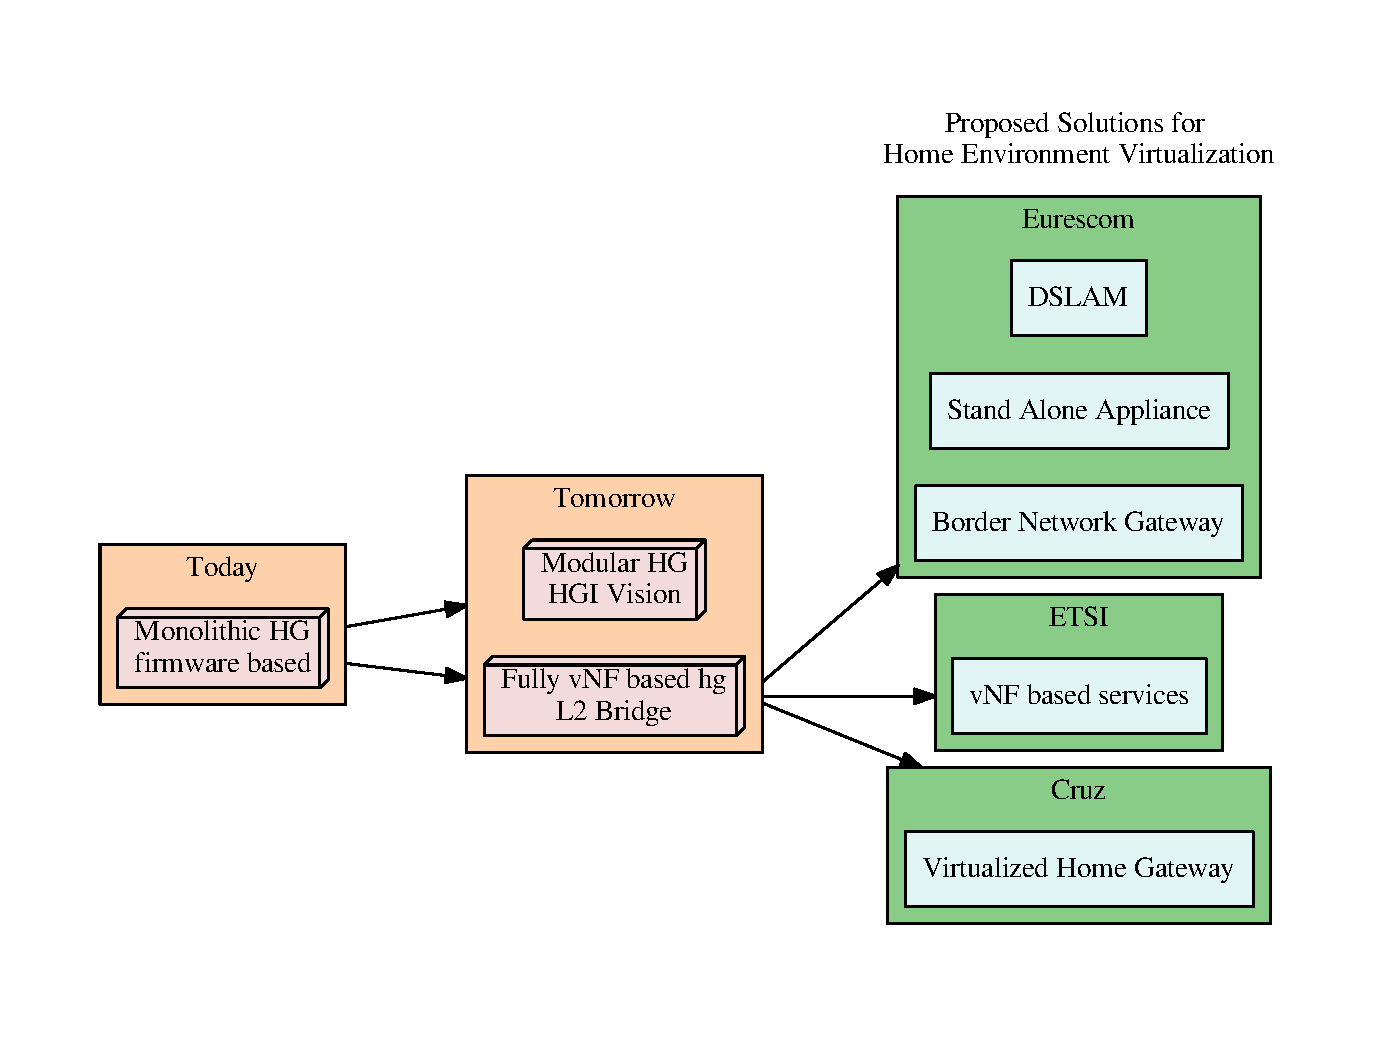
\includegraphics[width=0.45\textwidth]{fig/vhgtrends.pdf}
  \end{center}
  \caption{ Major trends for technical aspects of Home Gateway Virtualization
    \label{fig:trends}
  }
\end{figure}	

As a summary of the above-mentioned related works and their position in the landscape of Home Gateway Virtualization, Figure~\ref{fig:trends} depicts the overall context into which our proposal operates.
Building up on the latter approaches, this paper investigates an alternate, yet standard-based, migration path to a fully virtualized home environment, centered around a modular HG (using HGI open platform 2.0 with OSGi) cooperating with a carrier grade cloud computing architecture (NFV-ready and ETSI compliant), all this possible thanks to the introduction of a novel Surrogate vNF approach.




